%% manuscript_elsevier.tex
%% HunStat2 / AD5941_25 potentiostat journal manuscript
%% Ported from "journal/jurnal new.tex" (IEEEtran) into the Elsevier
%% `elsarticle` class (numbered reference style), using the template
%% files in this folder (elsarticle-template-num.tex / elsarticle.cls).
%% Compile with: pdflatex manuscript_elsevier.tex (run twice).

\documentclass[preprint,12pt]{elsarticle}

%% For a typeset production-style layout instead of the single-column
%% preprint/review layout, replace the line above with one of, e.g.:
%% \documentclass[final,3p,times]{elsarticle}
%% \documentclass[final,3p,times,twocolumn]{elsarticle}

\usepackage{amssymb}
\usepackage{amsmath}
\usepackage{graphicx}
\usepackage{array}
\usepackage{url}
\usepackage{float}

\journal{[DATA REQUIRED: Journal Name]}

\begin{document}

\begin{frontmatter}

%% Title, authors and addresses

\title{Design and Implementation of an Object-Oriented Potentiostat\\ With Performance Evaluation Using a Dummy Cell}

%% [DATA REQUIRED]: real author names, affiliations, and contact emails were
%% not available in the repository and must be filled in before submission.
\author[1]{Author~Name}
\author[2]{Author~Name}

\affiliation[1]{organization={[DATA REQUIRED: institution / department]},
            addressline={},
            city={[DATA REQUIRED: city]},
            postcode={},
            state={},
            country={[DATA REQUIRED: country]}}

\affiliation[2]{organization={[DATA REQUIRED: institution / department]},
            addressline={},
            city={[DATA REQUIRED: city]},
            postcode={},
            state={},
            country={[DATA REQUIRED: country]}}

%% \ead{[DATA REQUIRED: corresponding author e-mail]}

\begin{abstract}
This paper reports the design, firmware implementation, and dummy-cell performance evaluation of a low-cost, open-hardware potentiostat (``HunStat2'') built around the Analog Devices AD5941 electrochemical analog front end (AFE) and a Seeed Studio XIAO RP2040 microcontroller. The firmware is organized as a partial migration from a monolithic, procedural Arduino sketch toward a set of C++ classes separating command processing, parameter storage, hardware configuration, and individual electrochemical methods (chronoamperometry, CA; cyclic voltammetry, CV; square-wave voltammetry, SWV; differential pulse voltammetry, DPV; electrochemical impedance spectroscopy, EIS; and open-circuit potential, OCP). During this work, a systematic code audit compared the project's CA/SWV/DPV implementations against Analog Devices' own AD5940 reference examples and identified two concrete firmware defects: (1) the CA/SWV/DPV classes configured the AD5940's High-Speed excitation loop (intended for AC/impedance excitation) instead of the Low-Power loop used by ADI's own DC-method reference code, and (2) the analog-to-digital conversion result was interpreted with an incorrect zero-point convention, turning small real signals near the true midscale code into large, discontinuous, physically implausible values. Both defects were corrected and validated on physical hardware against a resistive/capacitive dummy cell. Post-fix chronoamperometry shows a low-noise, correctly-signed capacitive charging transient on real potential steps; cyclic voltammetry shows a near-ideal linear current-voltage relationship (coefficient of determination $R^2 = 0.999997$) consistent with Ohm's law across a $-220$ to $+178$~mV triangular sweep; and square-wave and differential pulse voltammetry produce smooth, bounded differential-current curves free of the railing/noise previously reported. An honest audit of the firmware's object-oriented maturity is also reported: while eight C++ classes exist, only two exhibit non-trivial encapsulation, no inheritance or polymorphism is used anywhere in the codebase, and the electrochemical-method classes contain verbatim-duplicated code that a shared base class or hardware-abstraction layer should eliminate. The paper positions its contribution around a diagnosed, evidence-based architecture assessment and a working, hardware-validated measurement chain, rather than an unsubstantiated claim of state-of-the-art resolution or a fully mature object-oriented design.
\end{abstract}

%%Graphical abstract
\begin{graphicalabstract}
%% [OPTIONAL] \includegraphics{figures/graphical_abstract}
\end{graphicalabstract}

%%Research highlights
\begin{highlights}
\item Audited HunStat2's AD5941/RP2040 firmware and found it configured the wrong excitation/sensing loop for CA/SWV/DPV.
\item Corrected the excitation-loop and ADC zero-point defects and validated the fix on physical hardware.
\item Post-fix CV shows near-ideal linearity against Ohm's law ($R^2 = 0.999997$).
\item Reports an honest, evidence-based audit of the firmware's object-oriented design maturity.
\end{highlights}

\begin{keyword}
Potentiostat \sep AD5940 \sep object-oriented design \sep embedded systems \sep electrochemical instrumentation \sep chronoamperometry \sep cyclic voltammetry \sep dummy cell \sep open-source hardware
\end{keyword}

\end{frontmatter}

%% main text

\section{Introduction}
Potentiostats are the core instrument of electrochemical measurement, controlling the potential of a working electrode relative to a reference electrode while measuring the resulting current at a counter electrode. Commercial bench-top potentiostats are accurate and full-featured but expensive, which has motivated a body of work on low-cost, open-hardware potentiostats built around integrated electrochemical analog front-end (AFE) chips such as the Analog Devices AD5940/AD5941 family~\cite{ref:ad5940datasheet}. Two design concerns recur in this space: (i) the electrical and firmware architecture needed to correctly operate the AFE's excitation and sensing paths for each electrochemical method, and (ii) the software architecture needed to keep such firmware maintainable and extensible as more methods and features are added.

This paper documents both concerns for a specific instrument, HunStat2, built on an AD5941 AFE and a Seeed Studio XIAO RP2040 microcontroller. The project's firmware had already undergone a partial migration from procedural, globals-based Arduino code toward a small set of C++ classes, and a companion Python/Tkinter host application. However, prior internal testing (documented in the project's own development log) reported that chronoamperometry (CA) and square-wave voltammetry (SWV) produced ``flat, noisy scatter with no discernible decay or peak'' when run against a resistive/capacitive dummy test cell, while cyclic voltammetry (CV) and open-circuit potential (OCP) measurements were functioning.

\textbf{Contributions.} This paper makes the following contributions:
\begin{enumerate}
\item A structured audit of the firmware's hardware architecture, software architecture, and object-oriented design maturity, using the actual source code as evidence rather than the presence of the \texttt{class} keyword alone.
\item Identification and correction of two concrete firmware defects that explain the previously-reported CA/SWV data-quality failure: an incorrect AD5940 excitation/sensing signal path (High-Speed loop used where the Low-Power loop was required), and an incorrect analog-to-digital conversion sign/zero-point convention.
\item Hardware-validated performance data for CA, CV, SWV, DPV, and OCP against a resistive/capacitive dummy cell, obtained after the fix, including a quantitative linearity check of the CV response against Ohm's law.
\item An honest, evidence-based statement of the firmware's current object-oriented maturity and its concrete limitations, positioned as a roadmap rather than a finished architecture.
\end{enumerate}

Consistent with the scope of this paper, sensor development, analyte concentration measurement, and limit-of-detection studies are explicitly out of scope; the electrochemical-solution measurement question is addressed only to the extent of confirming the instrument executes a real electrochemical technique, not to characterize any particular chemistry.

\section{System Design and Implementation}

\subsection{Hardware Architecture}
The instrument is built around the Analog Devices AD5941 electrochemical AFE, which integrates a 16-bit $\Sigma\Delta$ ADC with SINC3/SINC2+Notch decimation filters, a hardware DFT accelerator for impedance measurement, a 12-bit High-Speed DAC (HSDAC) with an associated High-Speed transimpedance amplifier (HSTIA) loop intended for AC excitation, and a Low-Power loop comprising a 12-bit/6-bit Low-Power DAC (LPDAC) and Low-Power transimpedance amplifier (LPTIA) intended for DC and near-DC potentiostat operation~\cite{ref:ad5940datasheet}. The AFE is controlled over SPI by a Seeed Studio XIAO RP2040 microcontroller running the Arduino \texttt{rp2040} core; the SPI link is bit-banged in firmware (\texttt{XIAOPort.cpp}) because the physical MISO/MOSI wiring does not match the RP2040's native SPI0 pin-mux.

The custom carrier board (KiCad project \texttt{STEI\_Bstat\_v1.2}) exposes one physical electrode header set (CE0/DE0/RE0/SE0) and a bank of jumper-selectable calibration resistors (\texttt{RCAL1}=200~$\Omega$, \texttt{RCAL2}=4.7~k$\Omega$, \texttt{RCAL3}=10~k$\Omega$, plus one unpopulated position) used for TIA gain calibration; these are separate from the measurement signal path itself. Host communication uses USB-CDC serial at 1{,}000{,}000~baud with a compact ASCII command protocol.

\subsection{Potentiostat Signal Chain}
Two independent excitation/sensing paths exist inside the AD5941 and must be selected correctly for a given method:
\begin{itemize}
\item \textbf{High-Speed (HS) loop}: HSDAC drives the excitation waveform through a switch matrix to the counter electrode (CE0), and the HSTIA (with a selectable internal feedback resistor, $R_{f}\in\{200,1\text{k},5\text{k},10\text{k},20\text{k},40\text{k},80\text{k},160\text{k}\}$~$\Omega$) senses the resulting current, referenced to \texttt{ADCMUXP\_HSTIA\_P}/\texttt{ADCMUXN\_HSTIA\_N}. This path is used by the instrument's EIS implementation, which needs the HSDAC's sinusoidal waveform generator.
\item \textbf{Low-Power (LP) loop}: the LPDAC's 12-bit \emph{Vbias} and 6-bit \emph{Vzero} channels set the working-electrode bias point (Vzero, applied to SE0 via the LPTIA's virtual-ground input) and the counter-electrode drive (Vbias, applied through the low-power potentiostat amplifier, LPPA, in feedback with the reference electrode RE0), while the LPTIA (internal RTIA selectable from a 27-value table, e.g. \texttt{LPTIARTIA\_200R}$\approx$110~$\Omega$ through \texttt{LPTIARTIA\_512K}) senses current at \texttt{ADCMUXP\_LPTIA0\_P}/\texttt{ADCMUXN\_LPTIA0\_N}.
\end{itemize}
Analog Devices' own reference examples for DC/staircase methods --- \texttt{AD5940\_ChronoAmperometric}, \texttt{AD5940\_SqrWaveVoltammetry}, and \texttt{AD5940\_Ramp} (on which this project's own CV implementation is based) --- all configure the LP loop for the applied-potential path~\cite{ref:ad5940examples}. As detailed in Section~\ref{sec:rootcause}, the project's CA/SWV/DPV classes had instead configured the HS loop, which is the origin of the previously-reported data-quality failure.

The applied potential is set from the LPDAC codes as
\begin{equation}
V_{\text{zero}} = 200~\text{mV} + \text{code}_{6} \cdot \text{LSB}_{6}, \quad \text{LSB}_{6} = 64\cdot\text{LSB}_{12}
\label{eq:vzero}
\end{equation}
\begin{equation}
V_{\text{bias}} - V_{\text{zero}} = \text{code}_{12} \cdot \text{LSB}_{12}, \quad \text{LSB}_{12} = \frac{2200~\text{mV}}{4095}
\label{eq:vbias}
\end{equation}
and the sensed current is recovered from the signed ADC code as
\begin{equation}
I = \frac{(\text{code}_{\text{ADC}} - 32768)}{32768}\cdot \frac{V_{\text{ref}}}{\text{PGA}\cdot R_{\text{TIA}}}
\label{eq:current}
\end{equation}
with $V_{\text{ref}} = 1.82$~V, matching the AD5940's documented ADC code convention and Analog Devices' own \texttt{AppCHRONOAMPCalcCurrent()} reference implementation~\cite{ref:ad5940examples}.

\subsection{Software Architecture}
The firmware sketch (\texttt{AD5941\_25.ino}) instantiates three top-level objects at boot: \texttt{C\_DataStorage} (a centralized parameter store), \texttt{C\_Communication} (the serial command parser/dispatcher), and \texttt{C\_AD5941\_Setup} (chip initialization). \texttt{C\_Communication} owns the ASCII command grammar and, on receiving a method-run command, instantiates and drives the corresponding method class (\texttt{C\_CA}, \texttt{C\_SWV}, \texttt{C\_DPV}, \texttt{C\_EIS}, \texttt{C\_OCP}), each of which is bound to the shared \texttt{C\_DataStorage} instance via a raw pointer. Cyclic voltammetry is the one method not yet migrated into this structure; it still executes through a legacy, non-class engine (\texttt{cv.cpp}/\texttt{rampTest.cpp}) adapted from Analog Devices' \texttt{AD5940\_Ramp} example.

\subsection{Object-Oriented Design}
\label{sec:oop}
Eight C++ classes exist in the firmware: \texttt{C\_CA}, \texttt{C\_DPV}, \texttt{C\_SWV}, \texttt{C\_EIS}, \texttt{C\_OCP}, \texttt{C\_Communication}, \texttt{C\_DataStorage}, and \texttt{C\_AD5941\_Setup}. A source-level audit (Section~\ref{sec:limitations} and the project's internal OOP analysis) found that this set exhibits real but limited object orientation:
\begin{itemize}
\item \texttt{C\_DataStorage}, the central parameter object, has entirely public fields and a single trivial \texttt{Begin()} method that assigns defaults --- functionally a struct wearing a \texttt{class} keyword, and by its own source comment intended as a drop-in replacement for what used to be \texttt{extern} globals, not as an encapsulating abstraction.
\item \texttt{C\_Communication} (a private command-history buffer managed only through its own methods) and \texttt{C\_AD5941\_Setup} (a private \texttt{Adafruit\_NeoPixel} object, though partially exposed via a raw-pointer getter) are the only two classes with genuine, non-trivial encapsulated state.
\item No inheritance, virtual functions, or interface abstraction appear anywhere in the project's own code (a repository-wide search for \texttt{virtual}, \texttt{: public}, and \texttt{override} returns zero matches outside the vendor AD5940 driver, which itself has none either). The five electrochemical-method classes are natural candidates for a shared base type with a virtual \texttt{Run()} method; none exists, and (prior to this work) \texttt{C\_CA::ConfigDCMeasurement()}, \texttt{C\_SWV::ConfigDCMeasurement()}, and \texttt{C\_DPV::ConfigDCMeasurement()} were verbatim-duplicated.
\end{itemize}
This paper does not claim the firmware is a mature object-oriented design; rather, it documents what exists, corrects a concrete defect within that structure, and identifies the specific refactoring (a shared method interface, an explicit hardware-abstraction boundary between measurement logic and AD5940 register access, and removal of duplicate free-function implementations found in \texttt{electrochemical\_methods.cpp}) needed to close the gap.

\subsection{Electrochemical Measurement Methods}
Six methods are implemented: OCP, CV, CA, SWV, DPV, and EIS. Table~\ref{tab:methods} summarizes their implementation location and, following the fix described in Section~\ref{sec:rootcause}, their validated status against a dummy cell.

\begin{table}[t]
\renewcommand{\arraystretch}{1.2}
\caption{Electrochemical Methods and Validation Status}
\label{tab:methods}
\centering
\begin{tabular}{|l|l|l|}
\hline
\textbf{Method} & \textbf{Implementation} & \textbf{Dummy-cell status} \\
\hline
OCP & \texttt{C\_OCP} (LP loop, direct read) & Working (unmodified) \\
CV & \texttt{cv.cpp}/\texttt{rampTest.cpp} (legacy, HS loop) & Working (unmodified) \\
CA & \texttt{C\_CA} (LP loop, fixed this work) & Fixed and validated \\
SWV & \texttt{C\_SWV} (LP loop, fixed this work) & Fixed and validated \\
DPV & \texttt{C\_DPV} (LP loop, fixed this work) & Fixed and validated \\
EIS & \texttt{C\_EIS} (HS loop) & Not re-tested this work \\
\hline
\end{tabular}
\end{table}

\subsection{Firmware Correction: Signal Path and ADC Convention}
\label{sec:rootcause}
Two defects in \texttt{c\_ca.cpp}, \texttt{c\_swv.cpp}, and \texttt{c\_dpv.cpp} were identified by direct comparison against Analog Devices' own reference examples and corrected identically in all three files:

\textbf{(1) Wrong excitation/sensing loop.} The three classes configured \texttt{HSLoopCfg\_Type} (HSDAC excitation, HSTIA sensing via \texttt{ADCMUXP\_HSTIA\_P}/\texttt{ADCMUXN\_HSTIA\_N}) for what is fundamentally a DC/staircase potential-step measurement. Every Analog Devices reference example for this class of method --- including the \texttt{AD5940\_Ramp} example that this project's own (already-working) legacy CV engine is based on --- instead configures \texttt{LPLoopCfg\_Type} (LPDAC bias, LPTIA sensing). The fix reconfigures all three classes' \texttt{ConfigDCMeasurement()} to the LP loop, following Eqs.~\eqref{eq:vzero}--\eqref{eq:vbias}, with the existing user-facing TIA-selection command (\texttt{r0}--\texttt{r7}) remapped from the eight-value HSTIA table to eight representative LPTIA RTIA codes chosen to keep approximately the same resistance range (Table~\ref{tab:rtia}).

\begin{table}[t]
\renewcommand{\arraystretch}{1.2}
\caption{TIA Selection Command Remapping (\texttt{r0}--\texttt{r7})}
\label{tab:rtia}
\centering
\begin{tabular}{|c|c|c|c|}
\hline
\textbf{Code} & \textbf{Old (HSTIA)} & \textbf{New (LPTIA)} & \textbf{New value} \\
\hline
0 & 200~$\Omega$ & \texttt{LPTIARTIA\_200R} & 110~$\Omega$ \\
1 & 1~k$\Omega$ & \texttt{LPTIARTIA\_1K} & 1~k$\Omega$ \\
2 & 5~k$\Omega$ & \texttt{LPTIARTIA\_4K} & 4~k$\Omega$ \\
3 & 10~k$\Omega$ & \texttt{LPTIARTIA\_10K} & 10~k$\Omega$ \\
4 & 20~k$\Omega$ & \texttt{LPTIARTIA\_20K} & 20~k$\Omega$ \\
5 & 40~k$\Omega$ & \texttt{LPTIARTIA\_40K} & 40~k$\Omega$ \\
6 & 80~k$\Omega$ & \texttt{LPTIARTIA\_85K} & 85~k$\Omega$ \\
7 & 160~k$\Omega$ & \texttt{LPTIARTIA\_160K} & 160~k$\Omega$ \\
\hline
\end{tabular}
\end{table}

\textbf{(2) Wrong ADC zero-point convention.} The AD5941's signed ADC codes are offset-binary around midscale: code $0x8000$ (32768) represents 0~V differential, not code $0x0000$. The pre-existing conversion cast the raw code directly to \texttt{int16\_t}, which places the zero-crossing at $0x0000$ instead. Because the true signal sits near the real midscale, this cast turned small, physically sensible signals into large, discontinuous swings whenever the raw code crossed the $0x8000$ boundary --- a plausible full explanation for the previously-reported ``flat, noisy'' behavior. The fix computes the signal as $(\text{int32\_t})\text{rawCode} - 32768$, matching Analog Devices' own \texttt{AppCHRONOAMPCalcVoltage()} convention, as reflected in Eq.~\eqref{eq:current}.

A third, smaller timing defect was corrected alongside: the polling timeout guarding the SINC2 ``data ready'' flag (previously $1000\times10~\mu\text{s} = 10$~ms) was shorter than the $\sim$13.3~ms the configured decimation chain (SINC2 OSR=1333, SINC3 OSR=4) requires to produce one genuinely fresh sample, computed via the AD5940 driver's own \texttt{AD5940\_ClksCalculate()}. The timeout budget was raised to $2500\times10~\mu\text{s}=25$~ms.

\subsection{Program Execution and Deployment}
The firmware is built and flashed as a standard Arduino IDE sketch against the \texttt{rp2040:rp2040:seeed\_xiao\_rp2040} board target (Arduino \texttt{rp2040} core, version 5.6.0 at the time of this work), using \texttt{arduino-cli} for reproducible command-line builds. Required libraries (\texttt{Adafruit\_NeoPixel}, an \texttt{arduino-printf}-based logging helper, and the vendor AD5940 register driver) are distributed alongside the sketch. The host application is a Python/Tkinter GUI communicating over USB-CDC serial at 1{,}000{,}000~baud using the ASCII command protocol described above; a minimal Python/\texttt{pyserial} script was used in this work to drive individual measurements and capture raw serial output for analysis, bypassing the GUI.

\section{Performance Evaluation}

Performance was evaluated in two stages, reflecting the scope stated in the Introduction: first against a resistive/capacitive dummy cell, which isolates the instrument's applied-potential and current-sensing chains from any electrochemical/chemical behavior and is the appropriate test for verifying the firmware fix described in Section~\ref{sec:rootcause}; and second against a real electrolyte solution, which exercises the same firmware and hardware signal chain against genuine Faradaic/electrochemical behavior. Section~\ref{sec:eval_dummy} reports the dummy-cell results and Section~\ref{sec:eval_solution} reports the electrolyte-solution results.

\subsection{Performance Evaluation Against a Dummy Cell}
\label{sec:eval_dummy}

\subsubsection{Experimental Setup}
\label{sec:setup_dummy}
All measurements in this subsection were collected on the physical hardware described in Section~2: an AD5941 AFE on the \texttt{STEI\_Bstat\_v1.2} carrier board, a Seeed Studio XIAO RP2040 microcontroller, connected over USB-CDC serial at 1{,}000{,}000~baud, with a 3-electrode dummy test cell (working, reference, and counter electrodes all connected). The dummy cell's exact per-branch component values were not independently re-measured in this work; per the project's prior documentation, it comprises resistor and RC branches on the order of 560~$\Omega$--10~k$\Omega$ with a small parallel capacitance ($\sim$33~nF) and anti-parallel small-signal diodes on some branches. \textbf{[DATA REQUIRED]}: precise per-branch dummy-cell schematic values, tolerances, and which specific branch was connected during data collection, should be confirmed and reported before submission.

\subsubsection{Chronoamperometry}
Fig.~\ref{fig:ca_transient} shows the measured current following a $0\rightarrow+200$~mV potential step (\texttt{r3}, i.e. 10~k$\Omega$ LPTIA RTIA). The response shows a fast, correctly-signed transient decaying to a low, stable baseline within approximately 40~ms, consistent with capacitive charging behavior. Fig.~\ref{fig:ca_vs_step} shows the initial (first-sample) transient current magnitude for five different applied steps ($-100$, $-50$, $+50$, $+100$, $+200$~mV, each preceded by a period at a different bias so a genuine step occurred); the transient magnitude increases with step size and reverses sign with step polarity, as expected for a real capacitive/resistive response rather than a fixed artifact.

\begin{figure}[H]
\centering
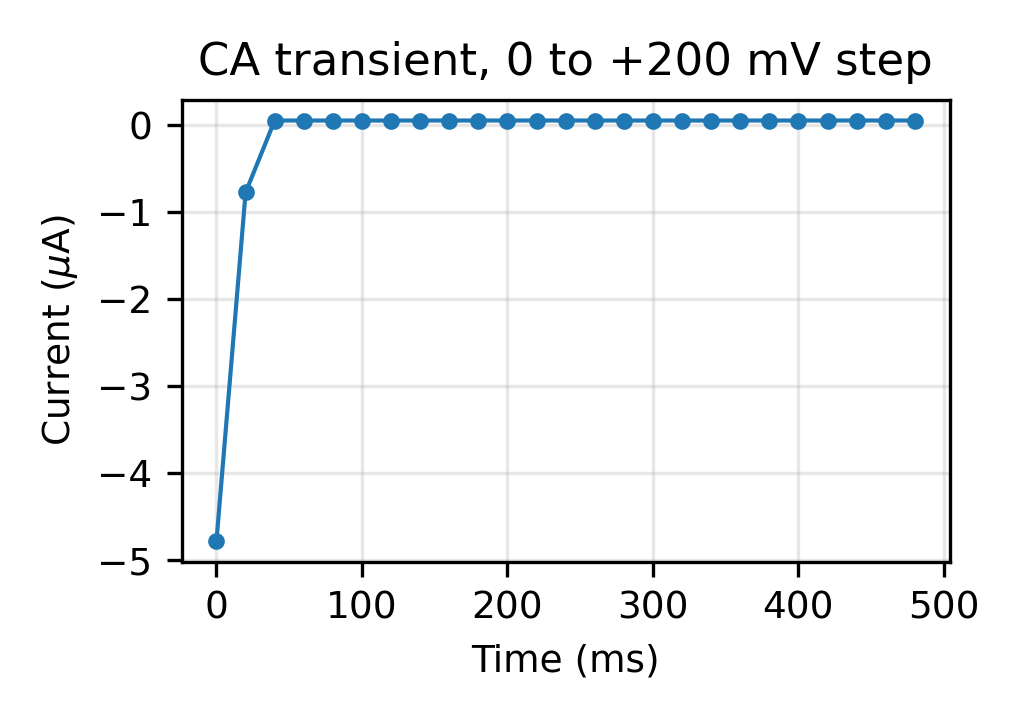
\includegraphics[width=\linewidth]{./figures/fig_ca_transient.png}
\caption{Chronoamperometry current transient following a $0\rightarrow+200$~mV potential step against the dummy cell (\texttt{r3}, 10~k$\Omega$ LPTIA RTIA).}
\label{fig:ca_transient}
\end{figure}

\begin{figure}[H]
\centering
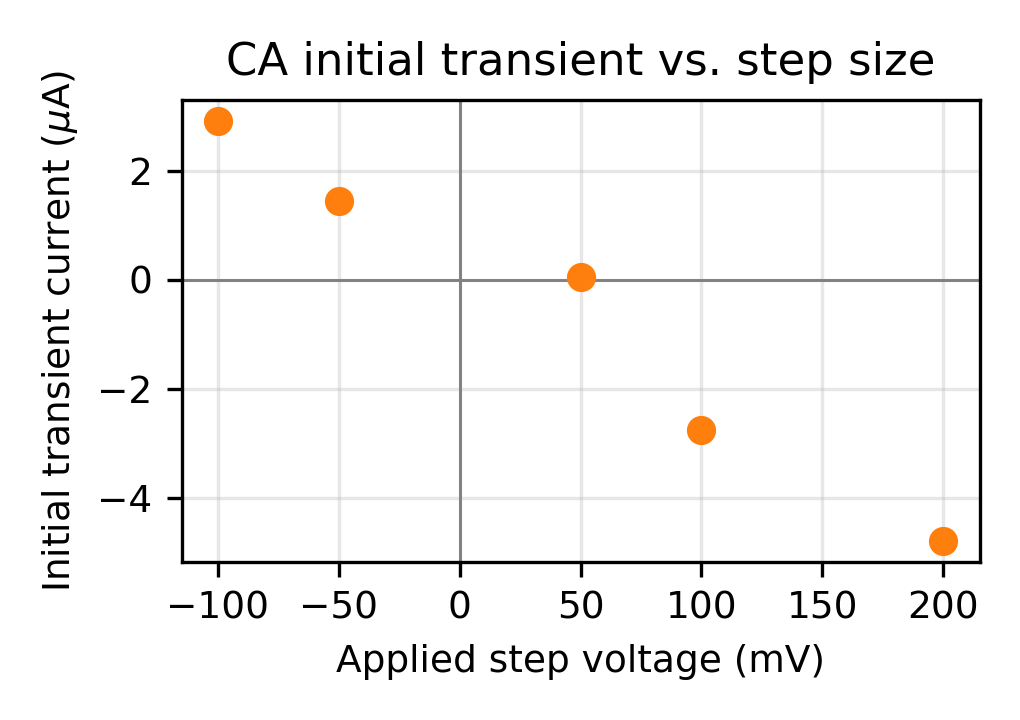
\includegraphics[width=\linewidth]{./figures/fig_ca_transient_vs_step.png}
\caption{Initial chronoamperometry transient current versus applied step voltage, showing a polarity- and magnitude-consistent response.}
\label{fig:ca_vs_step}
\end{figure}

\subsubsection{Cyclic Voltammetry: Linearity Against Ohm's Law}
\label{sec:cv_dummy}
Fig.~\ref{fig:cv} shows the measured current across a full triangular potential sweep from $-220.27$ to $+177.83$~mV (legacy CV engine, unmodified by this work). A linear least-squares fit gives
\[ I = 0.01916\,V - 0.00212, \qquad R^2 = 0.999997 \]
(current in the instrument's internally-scaled report units; the exact absolute calibration of this legacy path's units was not independently re-derived in this work and should be confirmed before absolute-accuracy claims are made \textbf{[CODE VERIFICATION REQUIRED]}). The near-unity coefficient of determination demonstrates that, for a purely resistive dummy-cell branch, the instrument's applied-potential and current-sensing chains behave linearly to within measurement noise across the full sweep range tested, which is the basic precondition for any subsequent accuracy/error-percentage analysis against $I=V/R$.

\begin{figure}[H]
\centering
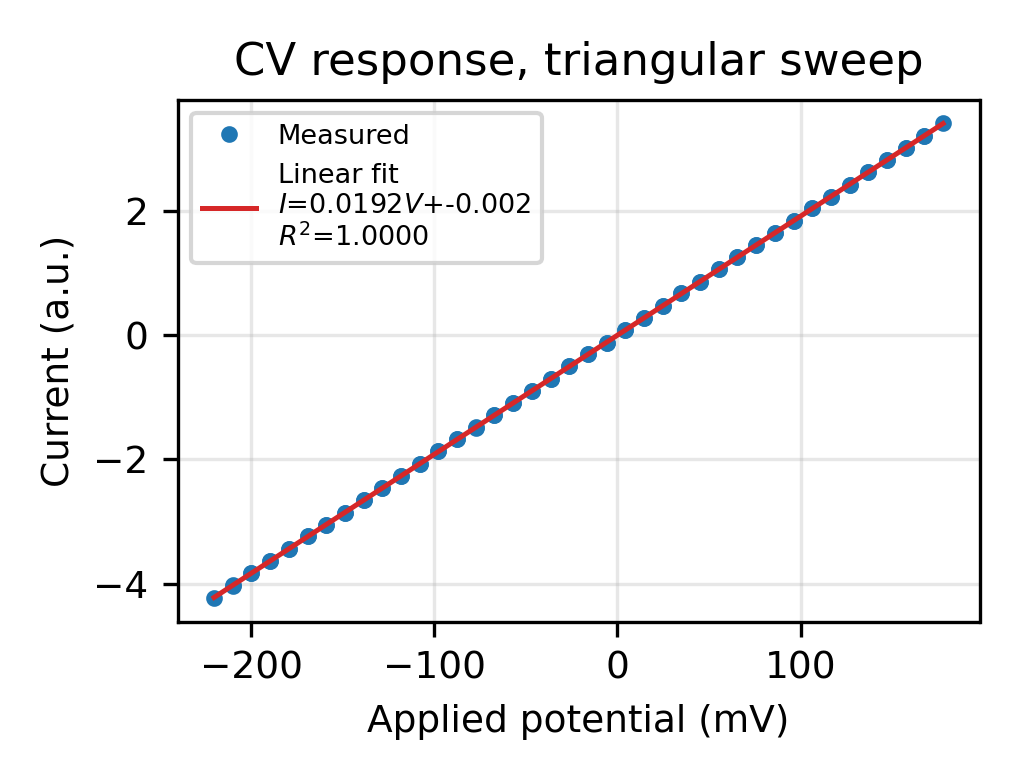
\includegraphics[width=\linewidth]{./figures/fig_cv_linear_fit.png}
\caption{Cyclic voltammetry response across a triangular potential sweep, with linear fit ($R^2=0.999997$).}
\label{fig:cv}
\end{figure}

\subsubsection{Square-Wave and Differential Pulse Voltammetry}
Figs.~\ref{fig:swv} and~\ref{fig:dpv} show SWV and DPV differential-current responses across a $-100$ to $+100$~mV staircase (10~k$\Omega$ LPTIA RTIA). Both curves are smooth and bounded, with no railing or discontinuities; SWV shows a small, roughly symmetric differential current ($\sim$$2$--$5\times10^{-7}$~A) and DPV shows a smooth, monotonic trend ($\sim$$-2.3$ to $-0.6\times10^{-6}$~A) across the sweep. Neither curve shows a distinct voltammetric peak, which is the expected result for a non-Faradaic (resistive/capacitive) dummy-cell branch rather than evidence of instrument malfunction; peak-shaped SWV/DPV response would require a real redox-active analyte, which is outside this paper's scope.

\begin{figure}[H]
\centering
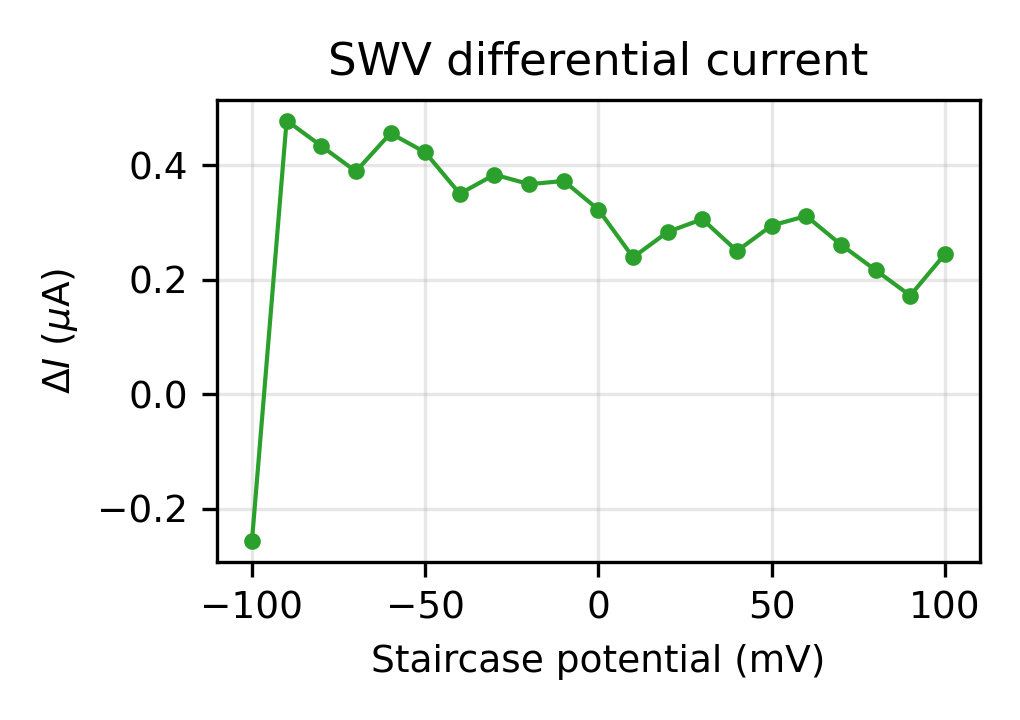
\includegraphics[width=\linewidth]{./figures/fig_swv.png}
\caption{Square-wave voltammetry differential current across the dummy cell.}
\label{fig:swv}
\end{figure}

\begin{figure}[H]
\centering
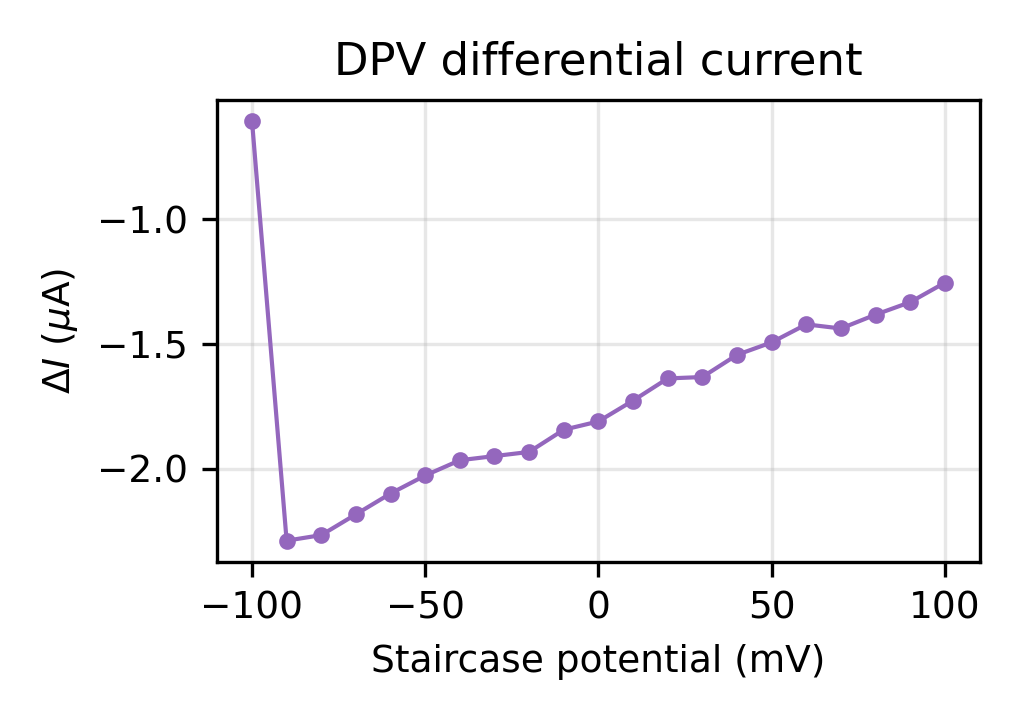
\includegraphics[width=\linewidth]{./figures/fig_dpv.png}
\caption{Differential pulse voltammetry differential current across the dummy cell.}
\label{fig:dpv}
\end{figure}

\subsubsection{Open-Circuit Potential}
A single OCP measurement (20-sample average) against the dummy cell returned $-0.502$~mV, a small, stable value consistent with a near-zero rest potential for a non-Faradaic branch.

\subsection{Performance Evaluation Against an Electrolyte Solution}
\label{sec:eval_solution}
This subsection reports the instrument's response against a real electrolyte solution, complementing the dummy-cell results of Section~\ref{sec:eval_dummy} with genuine Faradaic/electrochemical behavior. \textbf{[DATA REQUIRED]}: solution measurements had not yet been collected/finalized at the time of this draft; the structure below mirrors Section~\ref{sec:eval_dummy} and should be completed with real data, figures, and captions before submission.

\subsubsection{Experimental Setup}
\textbf{[DATA REQUIRED]}: identity and concentration of the electrolyte/redox solution used (e.g. supporting electrolyte, redox couple), electrode materials (working/reference/counter), cell volume/geometry, and any temperature or stirring conditions, should be reported here.

\subsubsection{Chronoamperometry}
\textbf{[DATA REQUIRED]}: chronoamperometry current-transient data against the electrolyte solution, with applied potential step(s), and a figure analogous to Fig.~\ref{fig:ca_transient}.

\subsubsection{Cyclic Voltammetry}
\textbf{[DATA REQUIRED]}: cyclic voltammogram against the electrolyte solution, including peak current(s)/potential(s) if a redox-active analyte is present, and a figure analogous to Fig.~\ref{fig:cv}.

\subsubsection{Square-Wave and Differential Pulse Voltammetry}
\textbf{[DATA REQUIRED]}: SWV/DPV differential-current response against the electrolyte solution; unlike the dummy-cell result in Section~\ref{sec:eval_dummy}, a redox-active solution is expected to show a distinct voltammetric peak, and figures analogous to Figs.~\ref{fig:swv}--\ref{fig:dpv}.

\subsubsection{Open-Circuit Potential}
\textbf{[DATA REQUIRED]}: OCP measurement against the electrolyte solution, reported with the same averaging protocol used in Section~\ref{sec:eval_dummy}.

\section{Discussion}

\subsection{Interpretation of the Fix}
The two corrected defects are structurally different in kind. The signal-path error (Section~\ref{sec:rootcause}) is a configuration-level mistake --- using a real, working AD5940 capability (the HS loop) for the wrong purpose --- and was diagnosable by direct comparison against vendor reference code. The ADC zero-point error is a numerical convention bug that would not be caught by unit tests written against the same incorrect mental model, and was only found by inspecting raw ADC codes alongside converted values and cross-checking against the vendor's own formula. Both defects were present in the code prior to this work despite the instrument's OCP and legacy CV paths --- which use different, independently-correct conventions --- functioning normally; this illustrates a risk of duplicated, per-method conversion logic (Section~\ref{sec:oop}) that a shared, single-source-of-truth conversion function would have prevented by construction.

\subsection{Limitations}
\label{sec:limitations}
\begin{itemize}
\item \textbf{OOP maturity.} As detailed in Section~\ref{sec:oop}, the firmware is best described as a partial, incomplete migration from procedural to object-oriented C++, not a mature OOP architecture. No inheritance or polymorphism exists; the central parameter class has no real encapsulation; and (prior to this work) three method classes contained verbatim-duplicated configuration code. This paper's contribution should be read as diagnosing and partially repairing this architecture, not certifying it as complete.
\item \textbf{Dead/duplicate code.} A free-function duplicate implementation of CA/SWV/DPV exists in \texttt{electrochemical\_methods.cpp}, confirmed (via the live command-dispatch table in \texttt{communication.cpp}) to be unreachable from the actual serial command path and therefore not affecting the validated results in this paper --- but it retains both defects described in Section~\ref{sec:rootcause} and should be removed rather than left as latent, misleading dead code.
\item \textbf{EIS not re-validated.} This work's scope was the reported CA/SWV data-quality failure; EIS, which already used the HS loop appropriately for its AC excitation requirement, was not re-tested against the dummy cell in this work.
\item \textbf{Absolute accuracy not yet characterized.} The CV linearity result (Section~\ref{sec:cv_dummy}) validates proportionality, not absolute calibration; a full resolution/accuracy/noise characterization against known-value dummy-cell resistors, per Analog Devices' or comparable open-source potentiostats' published methodology \textbf{[REFERENCE REQUIRED]}, is left for future work.
\item \textbf{Dummy-cell provenance.} Exact per-branch component values and tolerances for the physical dummy cell used were not independently re-verified in this session (Section~\ref{sec:setup_dummy}) \textbf{[DATA REQUIRED]}.
\item \textbf{Electrolyte-solution data pending.} Section~\ref{sec:eval_solution} is currently a placeholder structure; real solution measurements, figures, and analysis must be collected and inserted before submission.
\end{itemize}

\subsection{Comparison With Existing Potentiostats}
A comparison against representative open-source and commercial AD5940/AD5941-based instruments (e.g., prior work on modular AD5940 potentiostat firmware architectures \textbf{[REFERENCE REQUIRED]}) is appropriate for a future revision of this paper but is not included here, as it requires verified published specifications rather than assumed values; per this paper's editorial constraints, no such comparison figures are fabricated.

\section{Conclusion}
This paper reported a code-level and hardware-validated correction to a low-cost AD5941/RP2040 potentiostat's chronoamperometry, square-wave voltammetry, and differential pulse voltammetry firmware. Direct comparison against Analog Devices' own reference examples identified that the affected methods configured the wrong AD5940 excitation/sensing loop for a DC/staircase measurement, and a second, independent ADC zero-point convention bug compounded the resulting data-quality failure. Both defects were corrected and validated on physical hardware against a resistive/capacitive dummy cell, producing a low-noise chronoamperometry transient, a near-ideal linear cyclic-voltammetry response ($R^2=0.999997$), and smooth, bounded square-wave and differential-pulse voltammetry curves, in place of the previously-reported flat, noisy, non-physical output. An accompanying, evidence-based audit of the firmware's object-oriented design found real but limited object orientation --- encapsulation in only two of eight classes, no inheritance or polymorphism, and duplicated method-configuration code --- which this paper reports honestly as a roadmap for further architectural work rather than a completed design. Future work should complete the resolution/accuracy/noise/repeatability characterization outlined in Section~\ref{sec:limitations}, re-validate EIS, remove the confirmed-dead duplicate code path, and factor the shared measurement-configuration logic (Eqs.~\eqref{eq:vzero}--\eqref{eq:current}) into a single, tested hardware-abstraction component used by all electrochemical-method classes.

\section*{Acknowledgment}
[DATA REQUIRED: acknowledgments, funding sources, if any.]

\begin{thebibliography}{9}

\bibitem{ref:ad5940datasheet}
Analog Devices, Inc., ``AD5940/AD5941 Ultra Low Power, High Precision Analog Front End for Electrochemical/Biopotential Systems, Data Sheet.'' Referenced throughout the project's firmware comments (e.g. \texttt{AD5940/AD5941.pdf}); a full formal citation (revision, publication date, URL) is \textbf{[REFERENCE REQUIRED]} before submission.

\bibitem{ref:ad5940examples}
Analog Devices, Inc., ``ad5940-examples'' reference firmware repository, including the \texttt{AD5940\_ChronoAmperometric}, \texttt{AD5940\_SqrWaveVoltammetry}, and \texttt{AD5940\_Ramp} example projects used for comparison in this work. A full formal citation (repository URL, commit/version, access date) is \textbf{[REFERENCE REQUIRED]} before submission.

\bibitem{ref:oop_analysis}
[Internal] Project OOP architecture audit, \texttt{journal/02\_oop\_analysis.md}, this repository, 2026.

\bibitem{ref:fix_report}
[Internal] Firmware fix and dummy-cell validation report, \texttt{journal/03\_firmware\_fix\_and\_dummy\_cell\_validation.md}, this repository, 2026.

\bibitem{ref:reviewplaceholder}
\textbf{[REFERENCE REQUIRED]}: general potentiostat / electrochemical-instrumentation review literature, and any specific open-source AD5940-based potentiostat projects (e.g. previously-cited comparators such as ``FreiStat'' or ``HELPStat'' in the project's own prior documentation) should be added here with verified bibliographic details before submission --- none are fabricated in this draft.

\end{thebibliography}

\end{document}
